\section*{Supplementary Materials}

\section{World Model Design and Training}
\label{sec:supp-world-model}

The world model is an action-conditioned latent predictor optimized for efficient and robust rollout, rather than for photorealistic video generation. It is trained on heterogeneous, multi-embodiment data.



\subsection{Input Modalities and Latent Encoding}
\label{sec:supp-encoding}

The world model operates on a set of latent representations derived from multiple input modalities, consisting of visual observations, robot state, and action. All inputs are aligned temporally and encoded into a unified latent space before being processed by the spatio-temporal transformer.

\paragraph{Visual observations}
RGB observations are encoded independently at each timestep using a pretrained and frozen DINOv2 encoder. Each image is mapped to a grid of latent patch embeddings,
\[
x_t \in \mathbb{R}^{H \times W \times D_x},
\]
where $H \times W$ denotes the spatial resolution of the latent grid and $D_x$ is the per-patch embedding dimension. After projection, visual latents $x_t$ are denoted as $z_t$. When an associated decoder is available, it is used only for visualization of predicted futures and not for training.

\paragraph{Action and control signal inputs}
Robot actions and robot states are represented as per-timestep control tokens. Robot actions are expressed as end-effector delta motions in Cartesian space. These deltas are computed from observed state transitions rather than directly using low-level controller commands, allowing the model to remain agnostic to embodiment-specific control interfaces. Concretely, we treat each action/state component as a separate input key and encode it using a designated tokenizer, implemented as a lightweight embodiment-specific MLP, into latent tokens,
\[
c_{t,i} = f_i(a_{t,i}) \in \mathbb{R}^{A_i \times D_c},
\]
where $a_{t,i}$ denotes the $i$-th control component (action and, when available, state) at timestep $t$, and $f_i$ is the corresponding component-specific tokenizer. $A_i$ denotes the number of tokens produced by component $i$. The per-component tokens are then concatenated along the token dimension to form the control token sequence
\[
c_t = \big[ c_{t,1}, \ldots, c_{t,K} \big] \in \mathbb{R}^{A \times D_c}, \quad A=\sum_{i=1}^{K} A_i,
\]
with $K$ components provided by the embodiment.

\paragraph{Temporal alignment and batching}
Visual and control tokens are aligned at the timestep level. Given a sequence of length $T$, the model receives visual latents
\[
x \in \mathbb{R}^{B \times T \times S \times D_x}
\]
and corresponding control tokens
\[
c \in \mathbb{R}^{B \times T \times A \times D_c},
\]
where $S$ is the total number of visual tokens per timestep, aggregated across available views, and $A$ is the number of control tokens per timestep, which may vary across embodiments. These representations are inputs to the spatio-temporal transformer, which predicts future visual latents conditioned on past observations and the provided action/state sequence.


\paragraph{Projection to model dimension}
Before entering the transformer, both visual and control embeddings are linearly projected to a shared model dimension $D$. This allows the subsequent attention layers to operate in a unified embedding space while preserving the distinct structural roles of visual grid tokens and control tokens.


\subsection{Spatio-Temporal Transformer Architecture}
\label{sec:supp-st-arch}

Given the encoded visual and control tokens, the world model predicts future visual latents using a stack of spatio-temporal transformer layers. The transformer operates on two token streams: a grid of visual tokens and a set of per-timestep control tokens, and updates the visual stream through action-conditioned cross-attention.

\paragraph{Spatio-temporal transformer layers}

\begin{figure}[t]
  \centering
  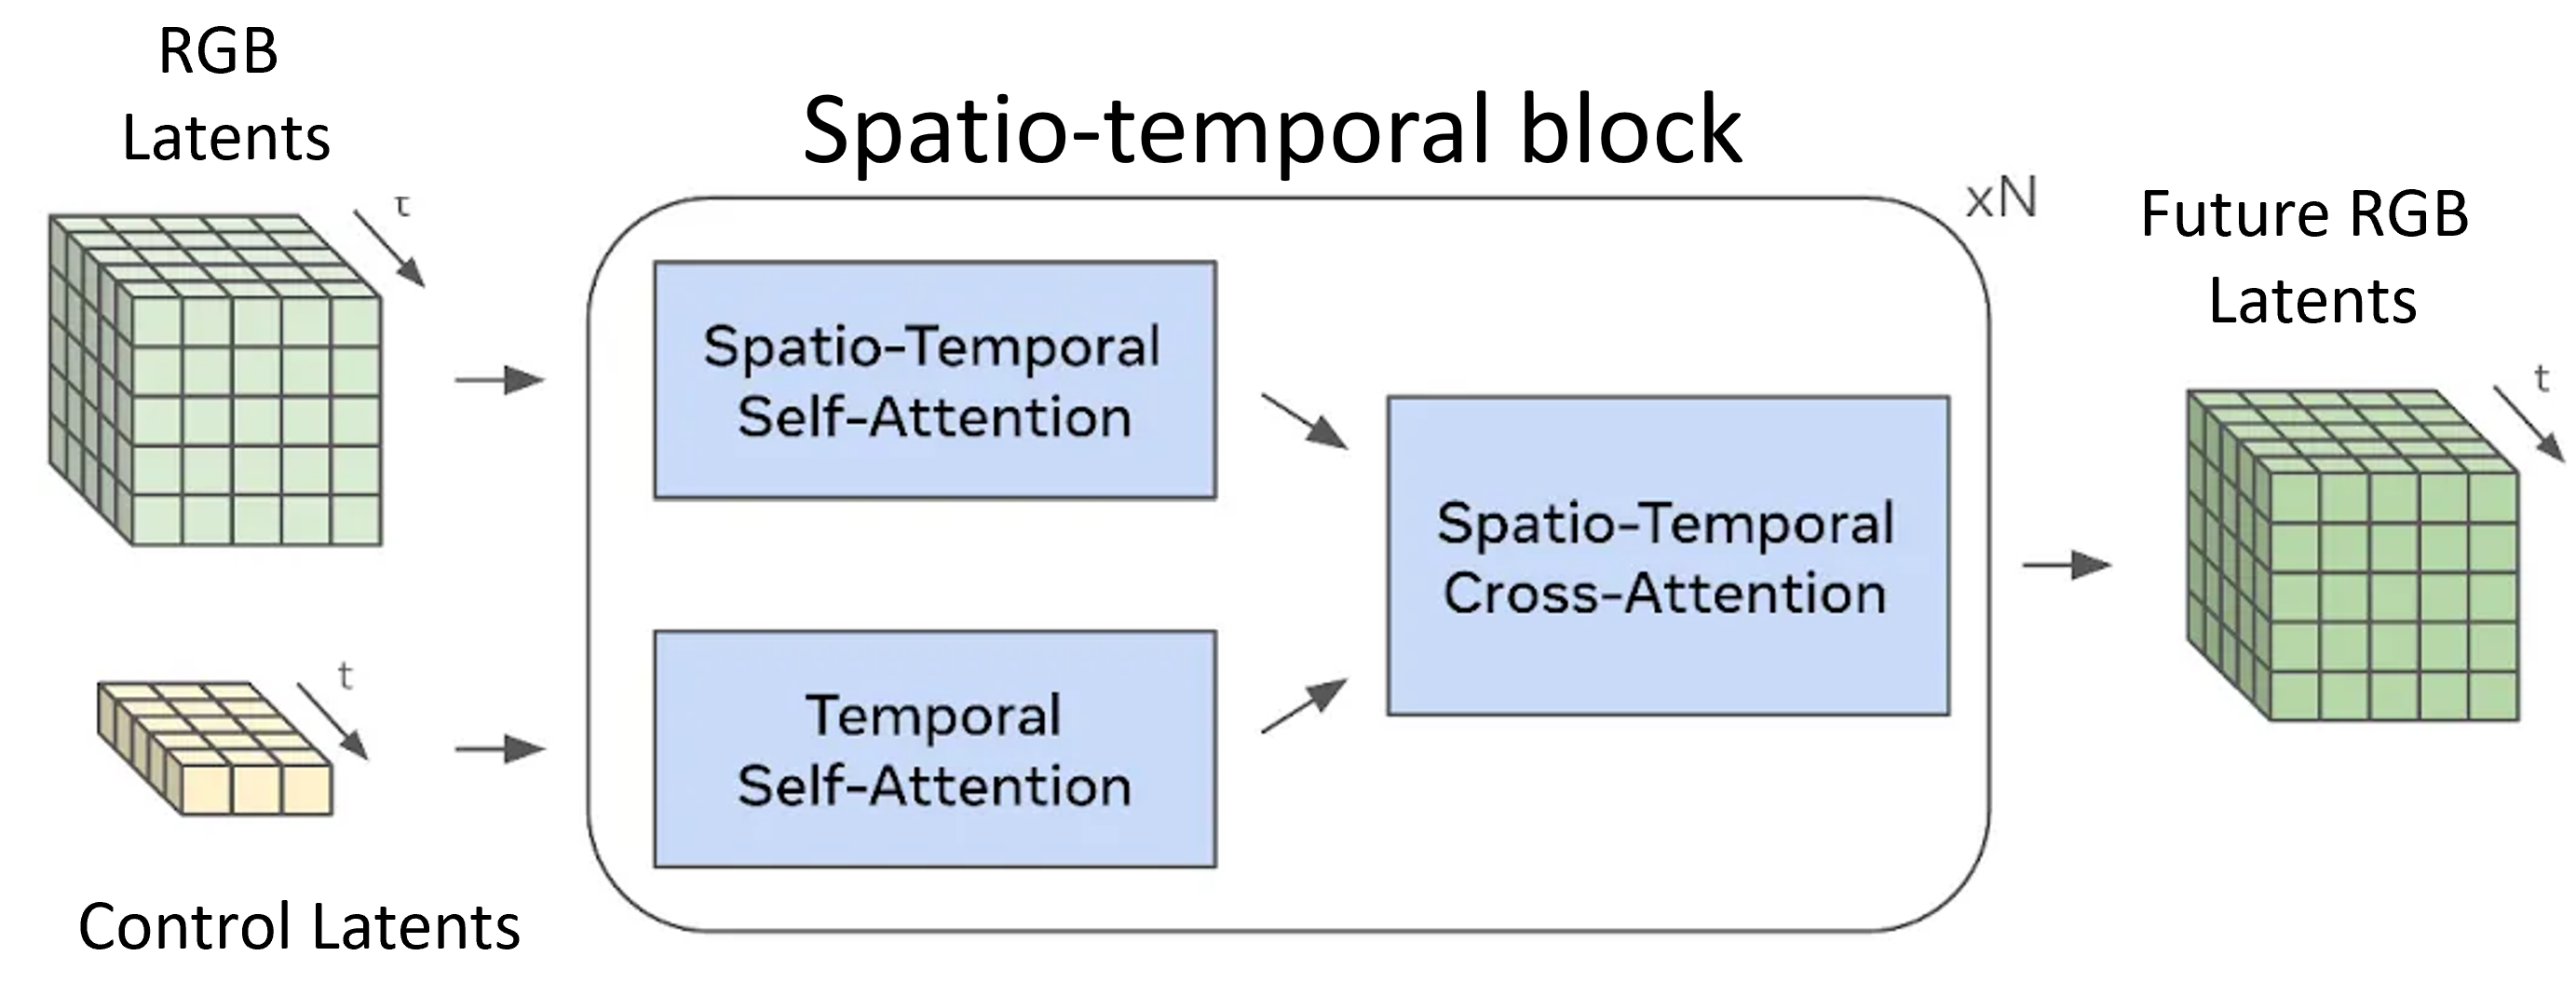
\includegraphics[width=\linewidth]{figures/st_block_new.png}
  \caption{\textbf{Spatio-temporal world model architecture.}}
  \label{fig:st_block}
\end{figure}


The transformer consists of $N$ repeated layers, each composed of three sequential blocks, as shown in Fig.~\ref{fig:st_block}: (i) spatio-temporal self-attention over visual tokens, (ii) temporal self-attention over control tokens, and (iii) spatio-temporal cross-attention from visual tokens to control tokens. Spatio-temporal self-attention is factorized into spatial attention applied independently within each timestep and causal temporal attention applied across timesteps at each spatial (or control) location. This factorization avoids full attention over all space-time tokens and improves computational efficiency for long-horizon rollouts. Action conditioning is introduced through cross-attention, where visual tokens act as queries and control tokens serve as keys and values in a time-aligned manner, which is shown in Fig.~\ref{fig:st-attention}.


% \paragraph{Positional encoding.}
% Rotary position embeddings (RoPE) are used to encode positional information without learned absolute embeddings. Separate RoPE parameterizations are applied for the temporal dimension, the two-dimensional spatial grid, and the context slots. RoPE is applied consistently in both self-attention and cross-attention to maintain temporal alignment between visual and context tokens.





\subsection{Train with Multi-Embodiment Data}
\label{sec:supp-mult-embodiment}

The world model is trained on data collected from multiple robot embodiments with heterogeneous sensory configurations and control interfaces. Differences across embodiments are handled at the input tokenization level, while all subsequent spatio-temporal dynamics parameters are fully shared.

\paragraph{Training datasets}
The world model is trained on a mixture of multi-embodiment manipulation datasets spanning both robot and human demonstrations. Our training corpus includes: (i) the DROID dataset collected on Franka platforms (76k trajectories, $\sim$350 hours), (ii) Franka subsets from RoboMIND, (iii) the EgoDex dataset consisting of human dexterous hand interactions, (iv) the AgiBot dual-arm manipulation dataset, and (v) an in-house teleoperation dataset containing approximately 1.2k trajectories collected on Franka arms equipped with dexterous hands.

In total, the combined dataset comprises on the order of $10^5$ trajectories and several hundred hours of interaction data. The data spans single-arm and dual-arm robots, parallel grippers and dexterous hands, as well as human hand demonstrations, covering diverse viewpoints and control interfaces. This heterogeneity enables the world model to learn embodiment-agnostic interaction dynamics while remaining compatible with varied sensory and action configurations.


\paragraph{Multi-view visual observations}

\begin{figure}[t]
  \centering
  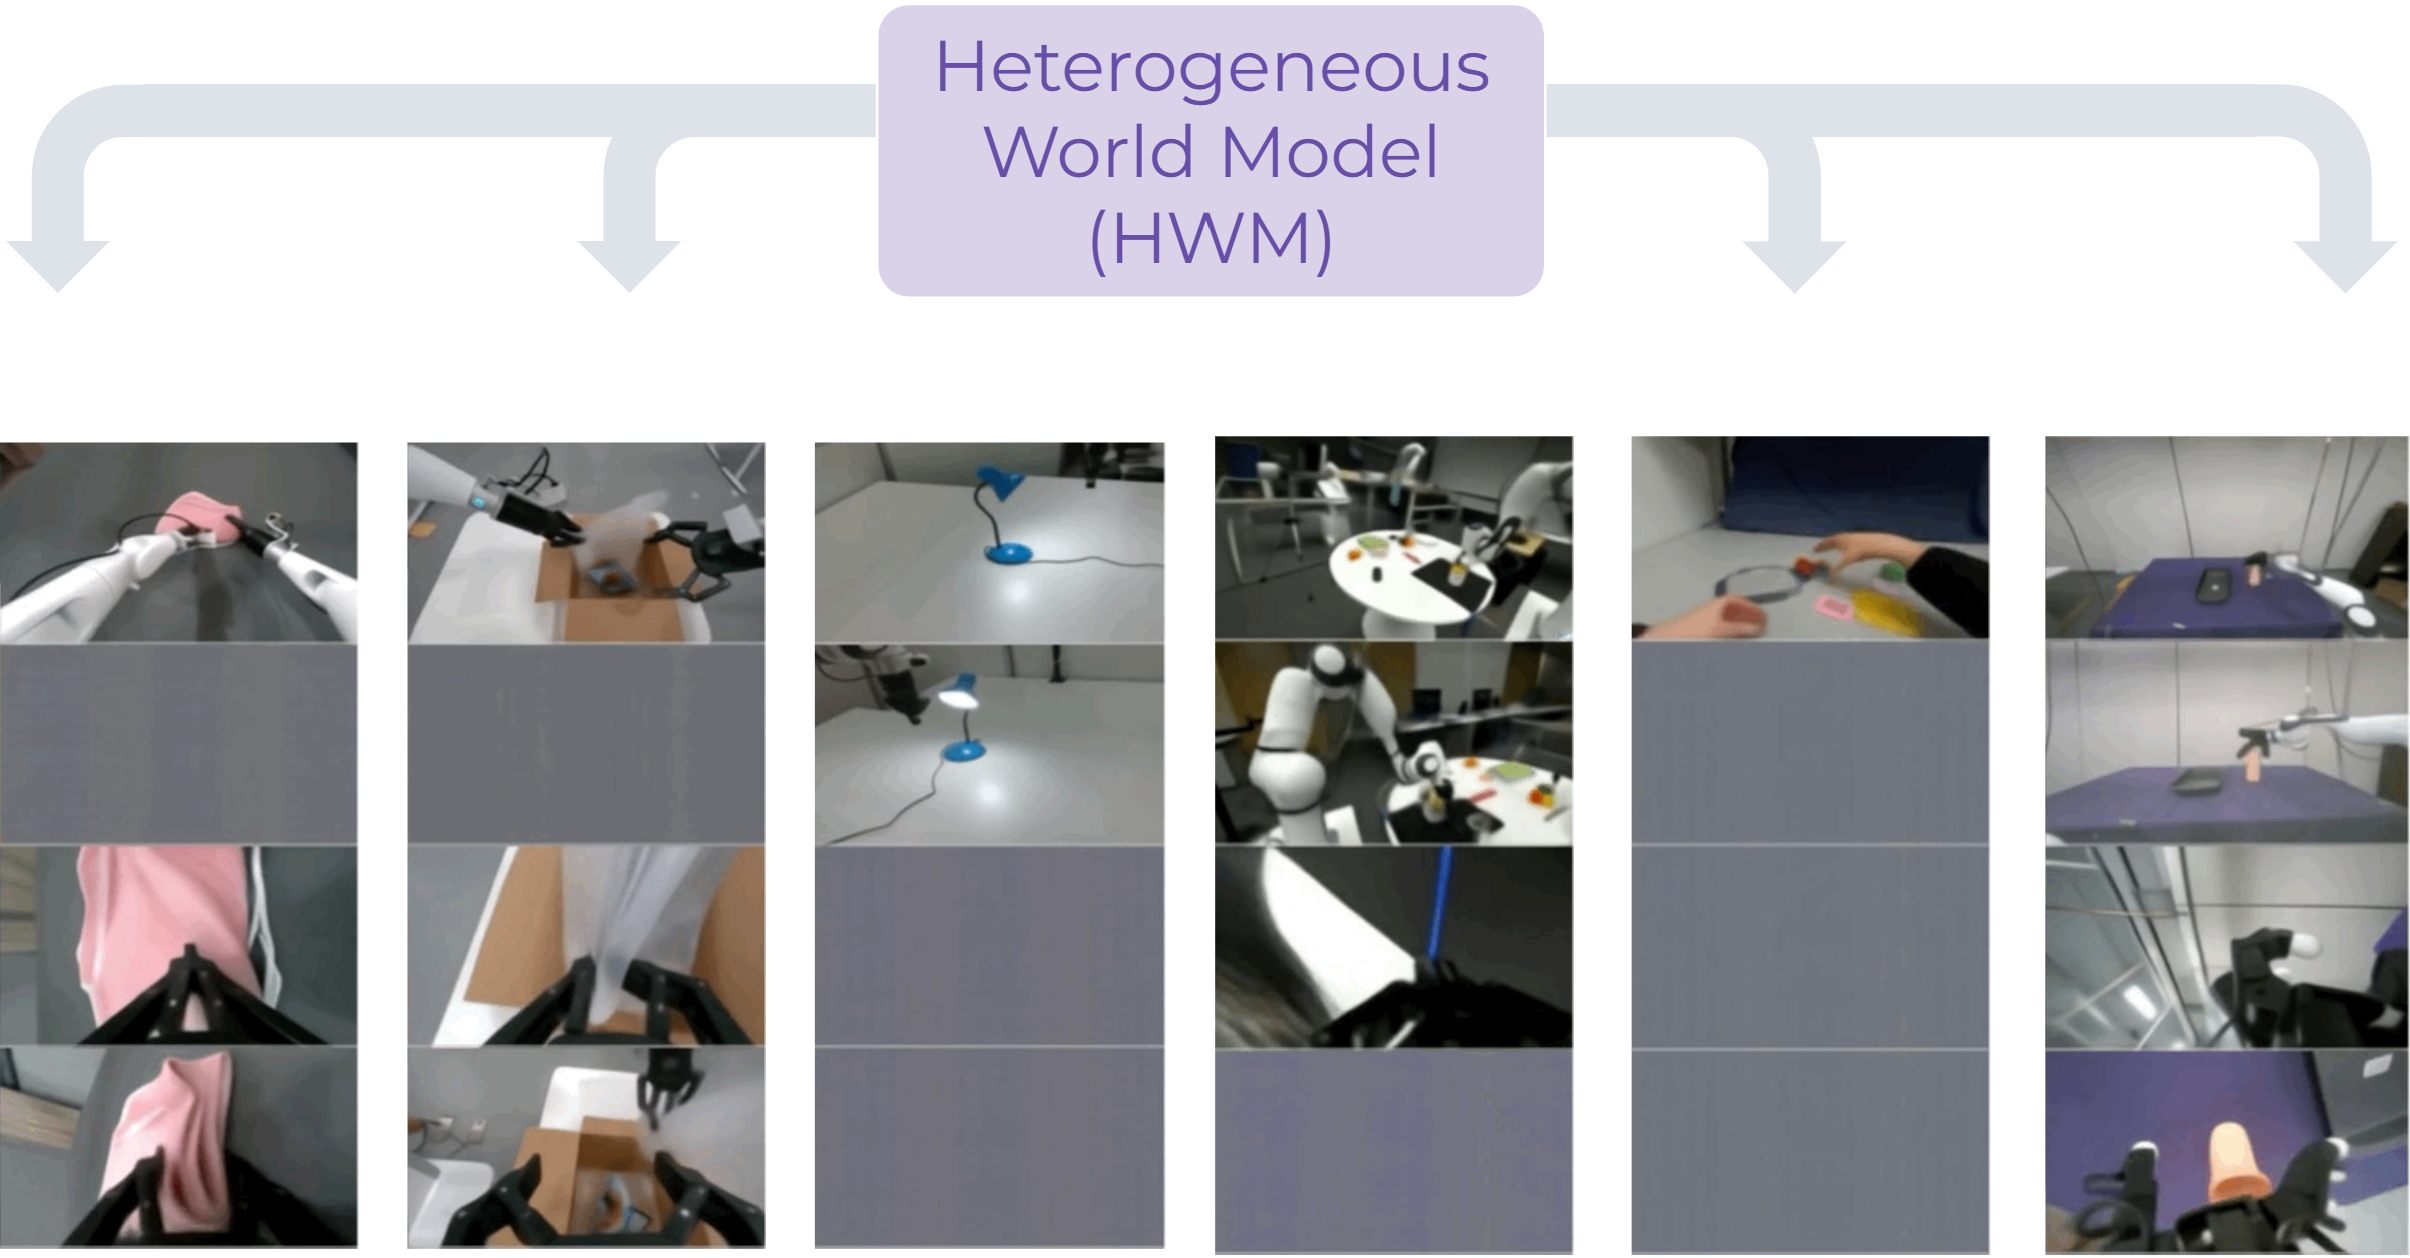
\includegraphics[width=\linewidth]{figures/multimodal_mask.png}
  \caption{\textbf{Mask strategy in multi-view data.}}
  \label{fig:multimodal_mask}
\end{figure}


Each timestep may include up to four RGB observations, consisting of two external views and two wrist-mounted views. Let
\[
\mathcal{V} = \{v_1, \dots, v_{|\mathcal{V}|}\}, \quad |\mathcal{V}| \leq 4
\]
denote the set of available viewpoints at a given timestep. Each view $v \in \mathcal{V}$ is independently encoded by a pretrained visual tokenizer into a grid of latent tokens. Since not all viewpoints are available for every timestep or embodiment, we employ token-level masking to handle missing observations, shown in Fig.~\ref{fig:multimodal_mask}. For each view $v$, a binary mask
\[
m_t^{(v)} \in \{0,1\}
\]
is expanded to all corresponding latent tokens and applied prior to the dynamics model. Masked tokens are zeroed out and excluded from loss computation, enabling the model to operate on partially observed multi-view inputs without introducing padded or hallucinated observations.




\paragraph{Shared dynamics across embodiments}
After tokenization and positional embedding, implemented via rotary position embeddings (RoPE), both visual tokens $x_t$ and control tokens $c_t^{(e)}$ are projected to a shared model dimension and processed by a spatio-temporal transformer. All transformer parameters are shared across embodiments; the only embodiment-specific components are the input tokenizers for actions and states. As a result, the model learns a unified latent dynamics representation while remaining compatible with heterogeneous sensory layouts and control interfaces.







\subsection{Autoregressive Rollout and Training Objective}
\label{sec:supp-rollout-loss}

\paragraph{Problem formulation}
Let $\mathbf{o}_{1:T}$ denote a sequence of observations and $\mathbf{a}_{1:T}$ the corresponding action/state tokens. After modality-specific tokenization (Sec.~\ref{sec:supp-encoding}), observations are represented as latent tokens
\[
\mathbf{z}_t \in \mathbb{R}^{S \times D},
\]
where $S$ is the number of visual tokens (aggregated across views) and $D$ is the shared model dimension. Actions and proprioceptive states are encoded as control tokens
\[
\mathbf{c}_t \in \mathbb{R}^{A \times D}.
\]

The world model learns a dynamics function
\[
f_\theta:\; (\mathbf{z}_{1:t}, \mathbf{c}_{1:t}) \;\rightarrow\; \hat{\mathbf{z}}_{t+1},
\]
implemented by the spatio-temporal transformer described in Sec.~\ref{sec:supp-st-arch}.

\paragraph{Sliding-window autoregressive rollout}
At both training and inference time, future observations are predicted autoregressively. Given an initial context of length $T_c$, predictions are generated sequentially:
\[
\hat{\mathbf{z}}_{t+1} = f_\theta(\mathbf{z}_{t-T_c+1:t},\; \mathbf{c}_{t-T_c+1:t}),
\]
where only the most recent $T_c$ steps are retained to bound memory and computation. Predicted tokens are appended to the context and used to predict subsequent steps:
\[
\hat{\mathbf{z}}_{t+k} = f_\theta(\hat{\mathbf{z}}_{t+k-T_c:t+k-1},\; \mathbf{c}_{t+k-T_c:t+k-1}).
\]

This sliding-window mechanism enables long-horizon rollout while maintaining fixed computational cost per step.

\paragraph{Teacher-forcing objective}
For one-step prediction, the model is trained using teacher forcing, where ground-truth observations are provided as input context. The loss is computed as mean squared error (MSE) in latent space:
\[
\mathcal{L}_{\text{1-step}}
= \frac{1}{T-1} \sum_{t=1}^{T-1}
\left\| \hat{\mathbf{z}}_{t+1} - \mathbf{z}_{t+1} \right\|_2^2.
\]

When modality masks are present (e.g., missing views), the loss is computed only over valid tokens:
\[
\mathcal{L}_{\text{1-step}}
= \frac{\sum m_{t,s}\,
\|\hat{\mathbf{z}}_{t+1,s} - \mathbf{z}_{t+1,s}\|_2^2}
{\sum m_{t,s}},
\]
where $m_{t,s}\in\{0,1\}$ denotes token validity.

\paragraph{Open-loop sampling objective}
To improve long-horizon stability, we additionally train the model using open-loop rollout. Starting from a short ground-truth context (typically one frame), the model generates predictions autoregressively for a rollout horizon $H_{\text{rollout}}$:
\[
\hat{\mathbf{z}}_{2:H_{\text{rollout}}+1}
=
\text{Rollout}_\theta
\!\left(
\mathbf{z}_1,\;
\mathbf{c}_{1:H_{\text{rollout}}}
\right).
\]

A final forward pass is then performed using the generated trajectory as context, and predictions are supervised against ground truth:
\[
\mathcal{L}_{\text{n-step}}
=
\frac{1}{H_{\text{rollout}}}
\sum_{t=1}^{H_{\text{rollout}}}
\left\|
\hat{\mathbf{z}}_{t+1}
-
\mathbf{z}_{t+1}
\right\|_2^2 .
\]

This objective encourages the model to remain stable under its own predictions and mitigates exposure bias.

\paragraph{Combined training objective}
During training, we alternate between teacher-forcing and sampling losses using a scheduled curriculum. At each optimization step, only one objective is active:
\[
\mathcal{L} =
\begin{cases}
\mathcal{L}_{\text{1-step}}, & \text{teacher-forcing step} \\
\mathcal{L}_{\text{n-step}}, & \text{sampling step}.
\end{cases}
\]

Both objectives are computed as mean squared error (MSE) in the latent space of the frozen visual encoder:
\[
\mathcal{L}
= \mathbb{E}\big[
\|\hat{\mathbf{z}} - \mathbf{z}\|_2^2
\big].
\]

No pixel-space reconstruction loss is used. Supervising predictions in latent space significantly reduces computational cost while preserving task-relevant dynamics required for rollout evaluation.



\paragraph{Training details and hyperparameters}
We train the world model using distributed data-parallel training on 384 NVIDIA H100 GPUs for approximately 2-3 days. Training follows the objectives described in Sec.~\ref{sec:supp-rollout-loss}, with frozen visual tokenizers and jointly optimized action/state tokenizers. All hyperparameters are listed in Table~\ref{tab:training-hparams}. 


\paragraph{Inference}
At deployment time, the world model operates purely autoregressively. Given past observations and candidate action sequences, future latent trajectories are rolled out and used for downstream evaluation without access to ground-truth future observations.




\begin{table}[h]
\centering
\small
\begin{tabular}{l l}
\toprule
\textbf{Hyperparameter} & \textbf{Value} \\
\midrule

\multicolumn{2}{l}{\textit{World Model Architecture}} \\
Model dimension $D$ & 1536 \\
Transformer layers & 8 \\
Attention heads & 24 \\
Visual latent dim $D_x$ & 1024 \\
Action/state latent dim & 16 \\


\midrule
\multicolumn{2}{l}{\textit{Context and Rollout}} \\
Training context length $T_c$ & 16 \\
Rollout horizon $H_{\text{rollout}}$ & 4 \\
% Autoregressive prediction & Yes \\
% Sliding window context & Yes \\

\midrule
\multicolumn{2}{l}{\textit{Optimization}} \\
Optimizer & AdamW \\
Learning rate & $1\times10^{-4}$ \\
Weight decay & $1\times10^{-2}$ \\
Gradient clipping & 1.0 \\
Batch size  & 384 \\
LR schedule & Cosine decay \\

\midrule
\multicolumn{2}{l}{\textit{Loss}} \\
Latent loss type & MSE (L2) \\
Teacher forcing & Yes \\
Sampling loss & Yes \\
Loss scheduling & Alternating curriculum \\



\bottomrule
\end{tabular}
\caption{Training hyperparameters for the spatio-temporal world model.}
\label{tab:training-hparams}
\end{table}





\subsection{World Model Rollout Visualization}
\label{sec:supp-rollout-vis}

We provide qualitative visualizations of autoregressive world model rollouts across multiple embodiments, viewpoints, and manipulation scenarios. In all visualizations, the model predicts future visual latents autoregressively conditioned on past observations and the provided action sequence. The rollout visualizations are shown in Fig.~\ref{fig:wm_rollout_all}.

Unless otherwise specified, rollouts are initialized from a single ground-truth observation frame, after which predictions are generated fully open-loop. We visualize decoded RGB observations obtained from the frozen visual tokenizer decoder for interpretability. Ground-truth and predicted frames are shown side-by-side for comparison.

\begin{figure}[t]
  \centering
  \includegraphics[width=\linewidth]{figures/wm_rollout_all.png}
  \caption{\textbf{World model rollout results.}}
  \label{fig:wm_rollout_all}
\end{figure}


% \subsubsection{Emergent Commonsense Interaction Behaviors}

\begin{figure}[t]
  \centering
  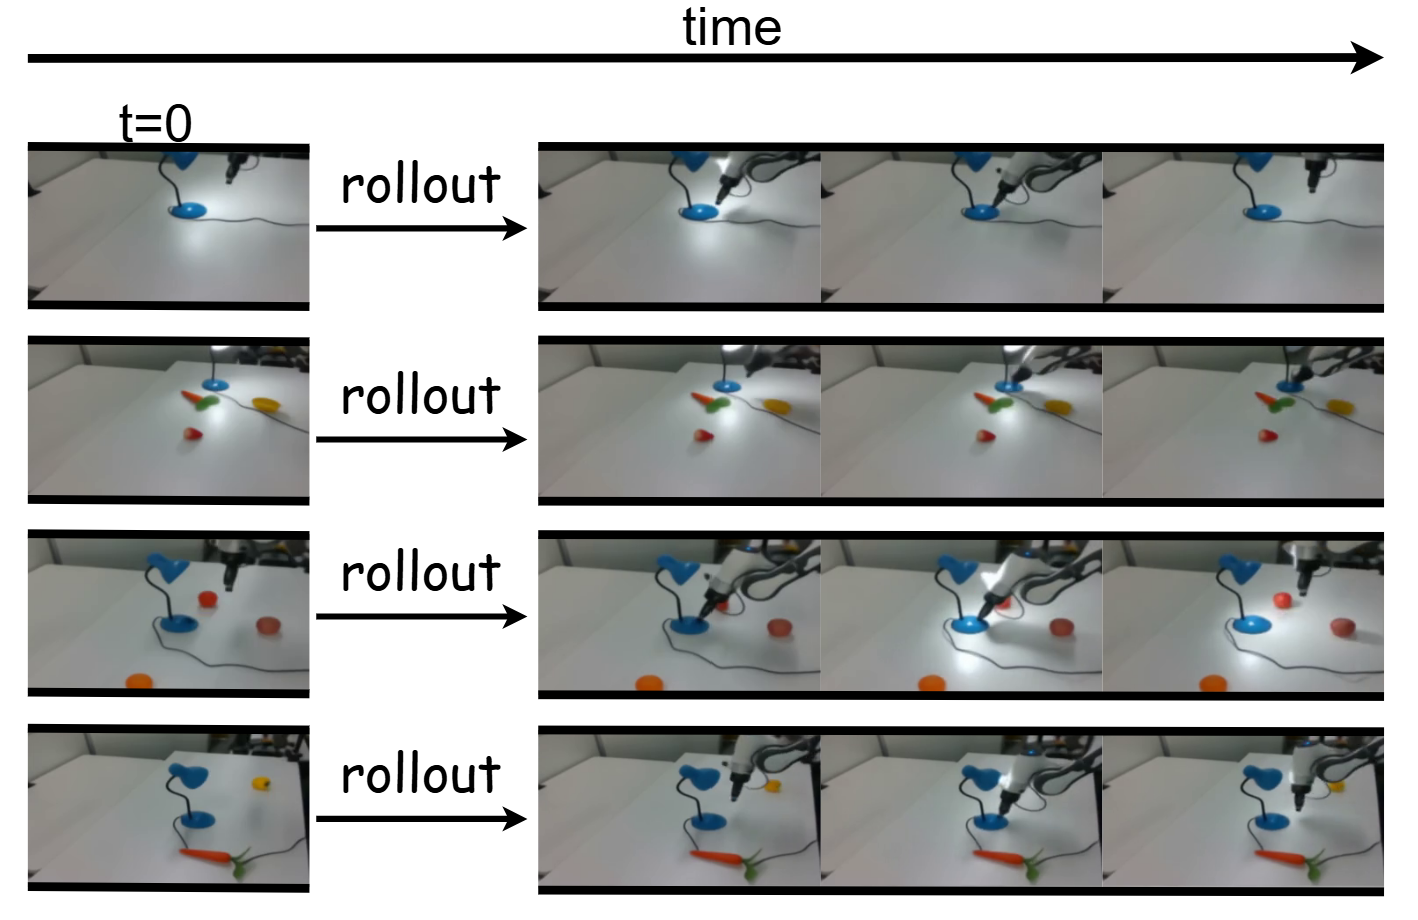
\includegraphics[width=\linewidth]{figures/light.png}
  \caption{\textbf{Functional interaction prediction.} When the robot toggles the light switch in imagination, the world model predicts corresponding changes in scene illumination.}
  \label{fig:light}
\end{figure}

Beyond low-level physical motion prediction, we examine whether the world model captures higher-level regularities of object functionality and human-designed interactions. As shown in Fig.~\ref{fig:light}, we consider imagined rollouts in which a robot interacts with a light switch. Conditioned on the toggling action, the model predicts a corresponding change in the environmental state, such as the light turning on or off. This behavior extends beyond immediate contact dynamics and reflects learned associations between object affordances and their functional effects. Such results suggest that the world model internalizes commonsense interaction patterns present in human environments, enabling it to anticipate functional outcomes of actions in addition to physical motion.


\section{Value Model and Trajectory Scoring}
\label{sec:supp-value}

\paragraph{Model choice}
To evaluate predicted rollouts during deployment-time steering, we adopt an off-the-shelf vision--language value model, Vision-Language-Action-Critic (VLAC), without any additional finetuning. VLAC is pretrained to estimate task progress between pairs of observations conditioned on a language instruction, producing a scalar progress score that reflects relative advancement toward task completion.

\paragraph{Rollout scoring formulation}
Given the current observation $o_t$ and a candidate action sequence $a_{t:t+H-1}$, the world model predicts a rollout of future observations
\[
\hat{o}_{t+1:t+H}.
\]

For a candidate rollout, we compute pairwise progress estimates between consecutive observations:
\[
s_{t+j}
=
\mathrm{VLAC}
\!\left(
\hat{o}_{t+j-1},
\hat{o}_{t+j},
l_{\mathrm{task}}
\right),
\qquad
\hat{o}_t = o_t ,
\]
where $l_{\mathrm{task}}$ denotes the language instruction.

\paragraph{Trajectory aggregation}
The trajectory-level score is obtained by summing progress estimates along the rollout:
\[
S
=
\sum_{j=1}^{H}
\mathrm{VLAC}
\!\left(
\hat{o}_{t+j-1},
\hat{o}_{t+j},
l_{\mathrm{task}}
\right).
\]

This score estimates how much the candidate action sequence advances the task specified by the language instruction. During deployment-time steering, multiple candidate action sequences are evaluated and ranked according to their trajectory scores, and the highest-scoring candidate is selected for execution. The value model operates on a single left-view RGB observation.



\section{Action Candidate Construction}
\label{sec:supp-candidates}

The pretrained $\pi_{0}$ policy outputs fixed-length action chunks in joint space with horizon $T=10$:
\[
\mathbf{q}_{t:t+T-1}.
\]
We convert these joint actions into end-effector Cartesian delta actions using forward kinematics (FK):
\[
\Delta \mathbf{p}_t = \mathrm{FK}(\mathbf{q}_{t+1}) - \mathrm{FK}(\mathbf{q}_t),
\]
resulting in Cartesian action chunks of the same length $T=10$.

In addition to policy-generated actions, we construct a set of hand-designed Cartesian action primitives, including directional motions (up, down, forward, backward, left, right) and gripper commands (open, close).


Each primitive defines a fixed Cartesian displacement (or gripper command), which is evenly distributed across the $T=10$ steps to form a temporally aligned action chunk.


\section{Hardware Setup and Evaluation Tasks}
\label{sec:supp-hardware}

\begin{figure}[t]
  \centering
  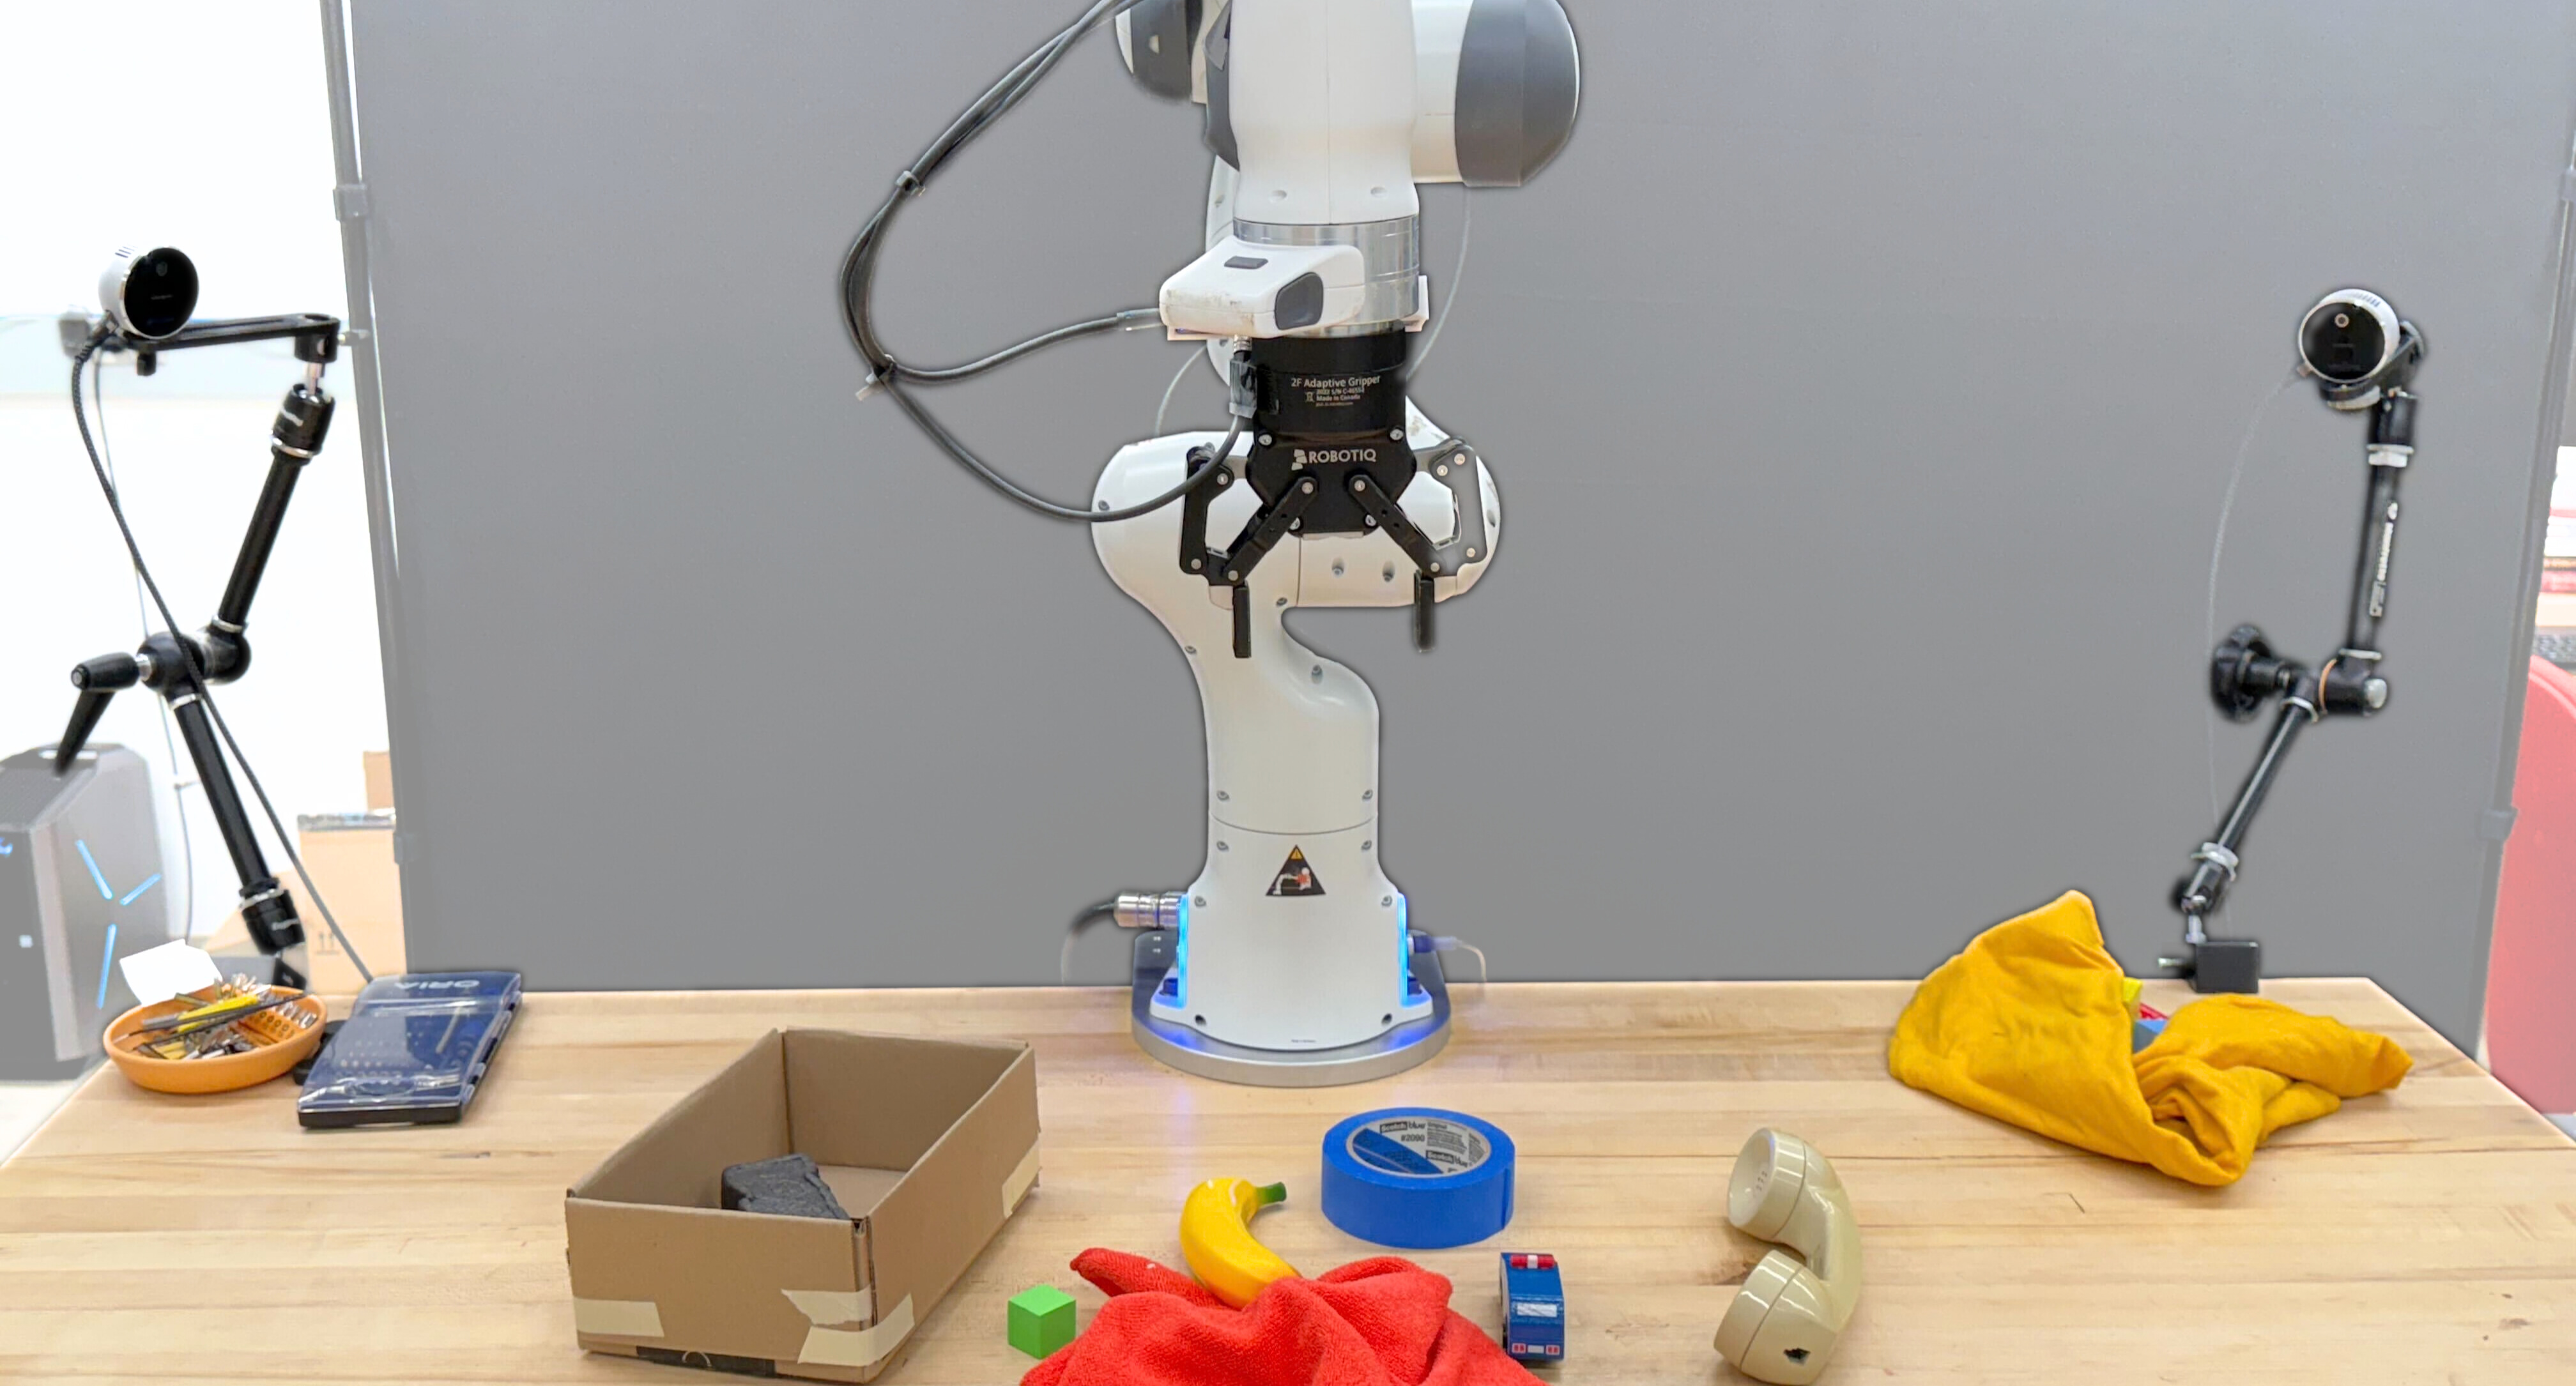
\includegraphics[width=0.9\linewidth]{figures/robot_edited.jpg}
  \caption{\textbf{Robot platform.}}
  \label{fig:robot_edit}
\end{figure}


 A visualization of the robot platform and camera configuration is shown in Fig.~\ref{fig:robot_edit}.


We evaluate real-world performance across two task families designed to assess generalization and language grounding under deployment conditions:

\begin{itemize}
    \item \textbf{Out-of-distribution (OOD) manipulation.} 
    The robot is instructed to manipulate novel objects not seen during training. Language instructions are:
    \begin{itemize}
        \item ``Pick up the \{phone\} and place it into the brown box.''
        \item ``Pick up the \{mustard\} and place it into the brown box.''
        \item ``Pick up the \{whiteboard eraser\} and place it into the black bowl.''
        \item ``Pick up the \{blue tape\} and place it into the black bowl.''
    \end{itemize}

    \item \textbf{Instruction following with distractors.} 
    The robot must identify the correct target object in the presence of visually similar distractors. Instructions and distractors are:
    \begin{itemize}
        \item ``Pick up the \{sponge\} and place it into the black bowl.''. The distractors are banana, police car toy, and pencil case.
        \item ``Pick up the \{banana\} and place it into the black bowl.'' The distractors are sponge, police car toy, and pencil case.
        \item ``Pick up the \{pencil case\} and place it into the brown box.'' The distractors are brush, can, and apple.
        \item ``Pick up the \{apple\} and place it into the brown box.'' The distractors are brush, can, and pencil case.
    \end{itemize}
\end{itemize}




% \section{Failure Modes}
% \label{sec:supp-failure}

% \subsection{World Model Hallucination}
% \label{sec:supp-hallucination}



% Magic grasp hallucination is a common failure mode occurs during contact-rich manipulation, where the world model predicts successful grasps despite failure in the real world. Figure~\ref{fig:magic_grasp} shows two examples in which the robot fails to grasp the object during execution, while the world model rollout incorrectly depicts the object as being grasped and lifted.

% \begin{figure}[h]
% \centering
% 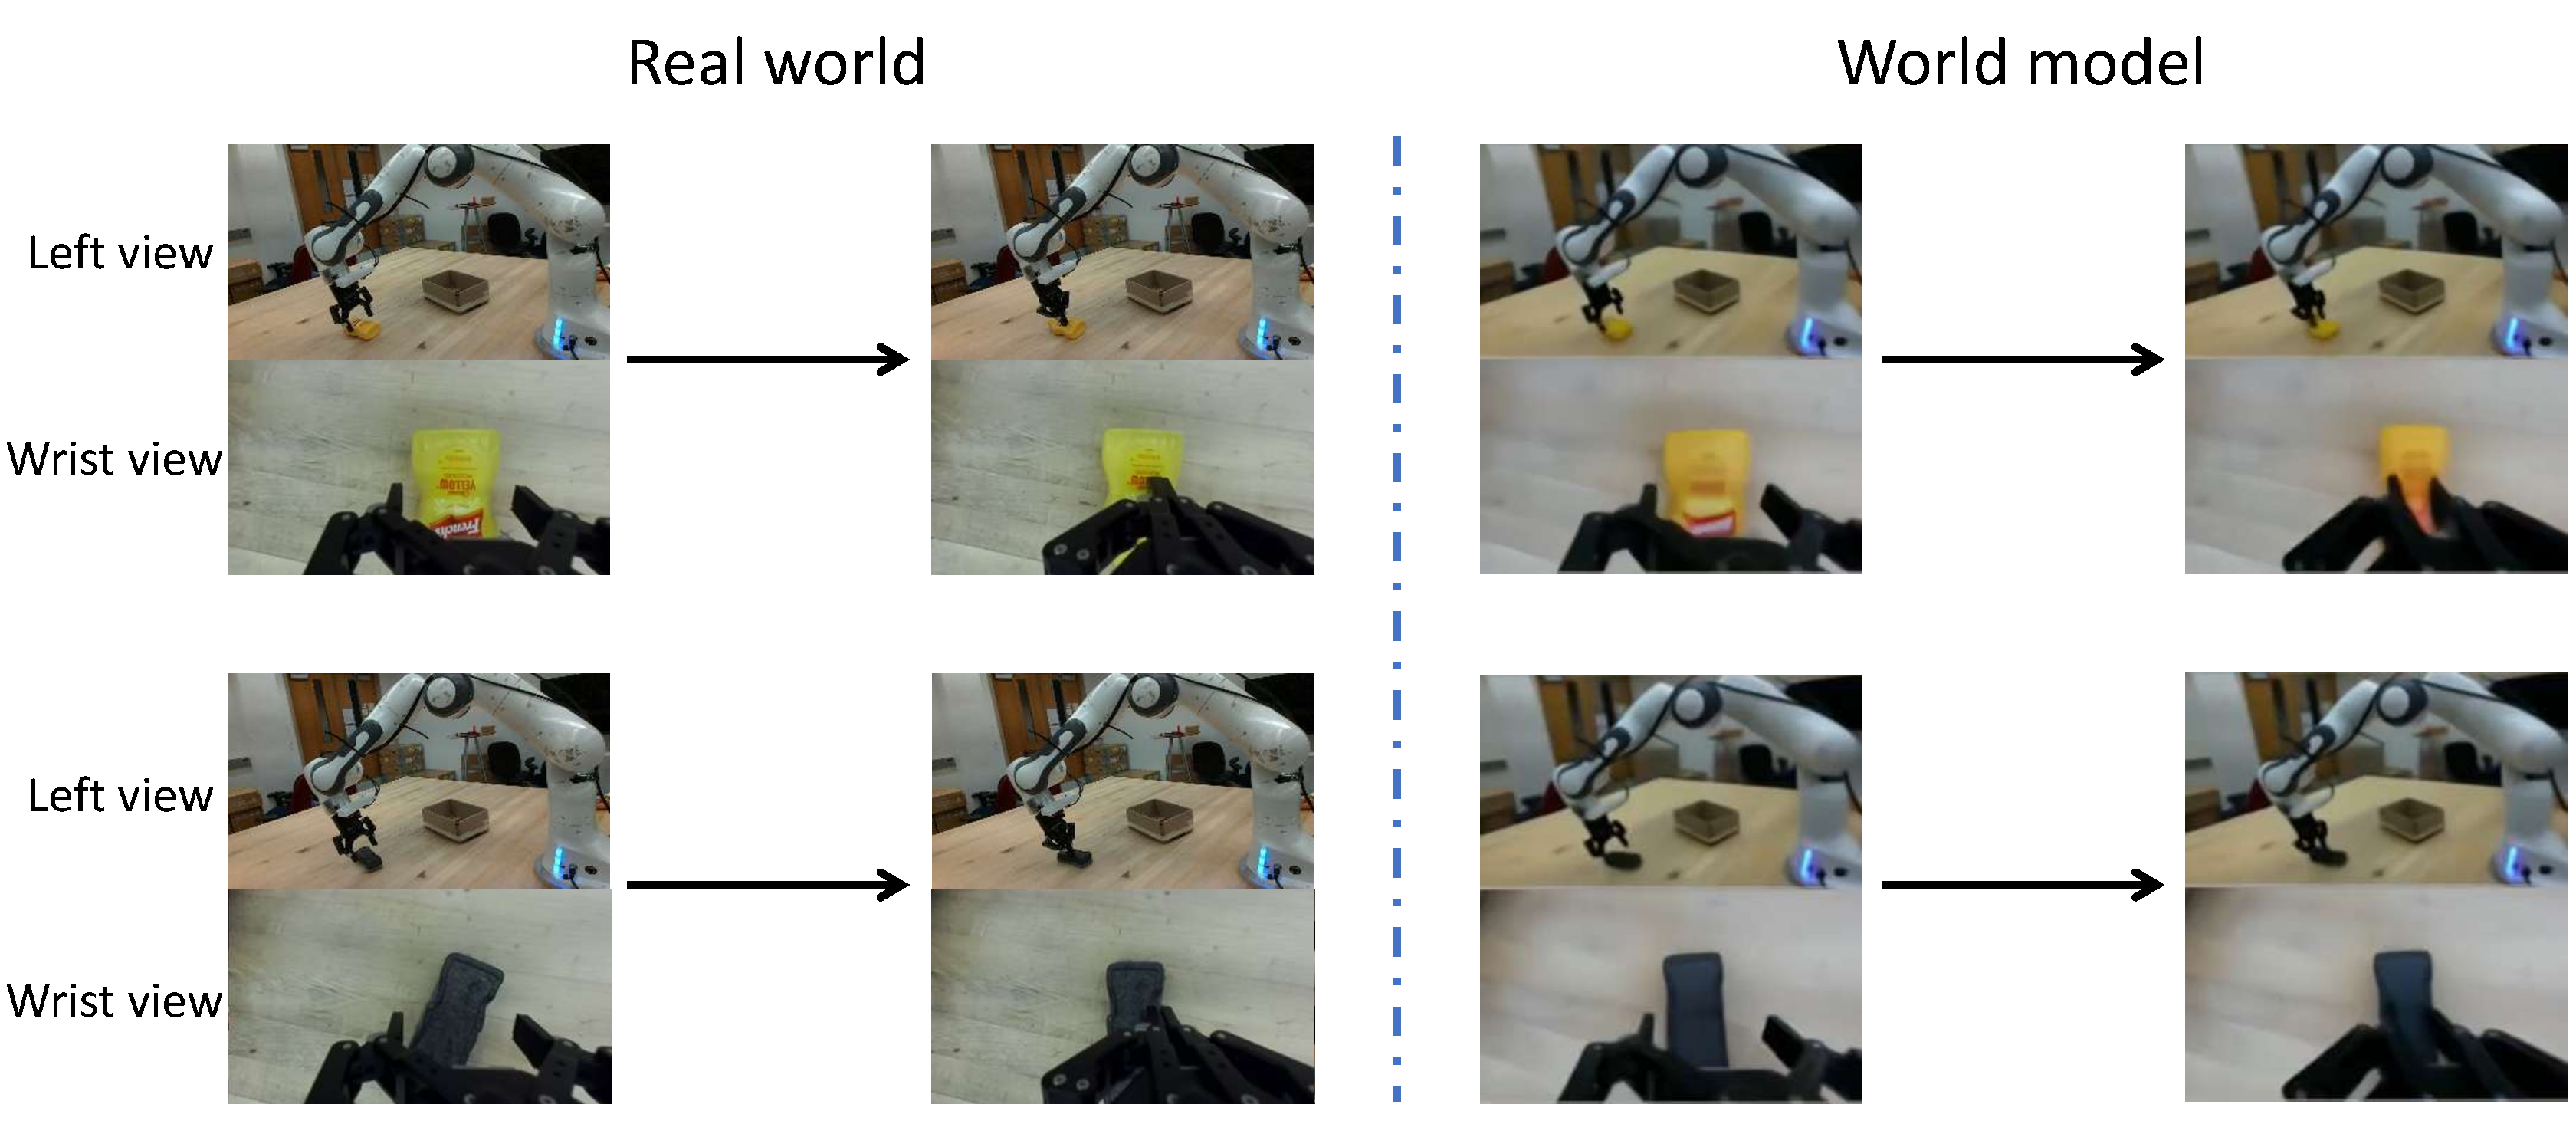
\includegraphics[width=\linewidth]{figures/wm_hallucinate.pdf}
% \caption{
%     \textbf{World model hallucination examples.}
%     Left: real-world execution where the object is not grasped. Right: world model rollout predicting a successful grasp.}
% \label{fig:magic_grasp}
% \end{figure}



% \subsection{Value Model Misranking}
% \label{sec:supp-value-misranking}

% \begin{figure}[h]
% \centering
% 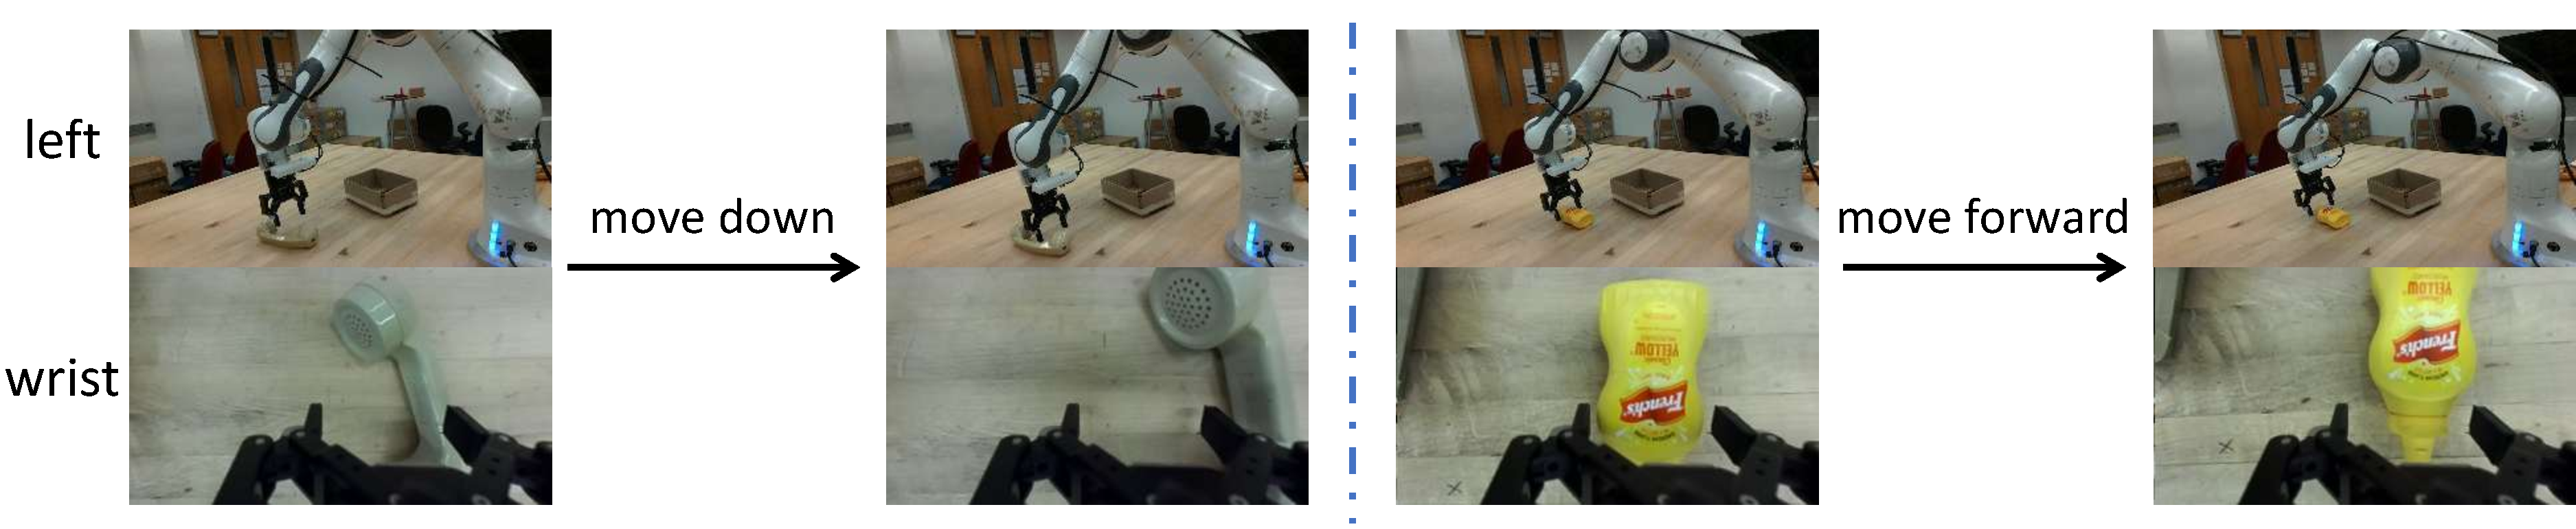
\includegraphics[width=\linewidth]{figures/misrank.pdf}
% \caption{
% \textbf{Value model misranking examples.}
% }
% \label{fig:value_misranking}
% \end{figure}




% We observe failure cases where the value model assigns higher scores to suboptimal action candidates, resulting in incorrect steering decisions during deployment. Figure~\ref{fig:value_misranking} illustrates two representative real-world examples.


% In the phone case, the selected action corresponds to a downward motion that brings the gripper closer to the object. However, this motion does not place the gripper in a grasp-ready pose. In the mustard case, the robot already reaches a grasp-ready pose, yet the value model favors a forward motion, causing the gripper to move away from the target object.



% We attribute these misranking failures primarily to limited visual observability in the value model input. The value model operates on a single left-view RGB observation, under which certain action outcomes appear visually ambiguous, leading to incorrect value ordering.








